\documentclass{standalone}
\usepackage{amsmath, amsfonts, amsthm}
\usepackage{siunitx}
\usepackage{graphicx}
\usepackage{tikz}
\usepackage{circuitikz}
\usetikzlibrary{patterns}
\usepackage{scalerel}
\usepackage{pict2e}
\usepackage{tkz-euclide}
\usetikzlibrary{calc}
\usetikzlibrary{arrows.meta}
\usetikzlibrary{shadows}
\usetikzlibrary{external}
\usetikzlibrary{decorations.pathmorphing}
\usetikzlibrary{shapes.geometric}
\usetikzlibrary{arrows,shapes.gates.logic.US,shapes.gates.logic.IEC,calc}
\usepackage{pgfplots}
\pgfplotsset{compat=newest}
\usepgfplotslibrary{statistics}
\usepgfplotslibrary{fillbetween}

\begin{document}
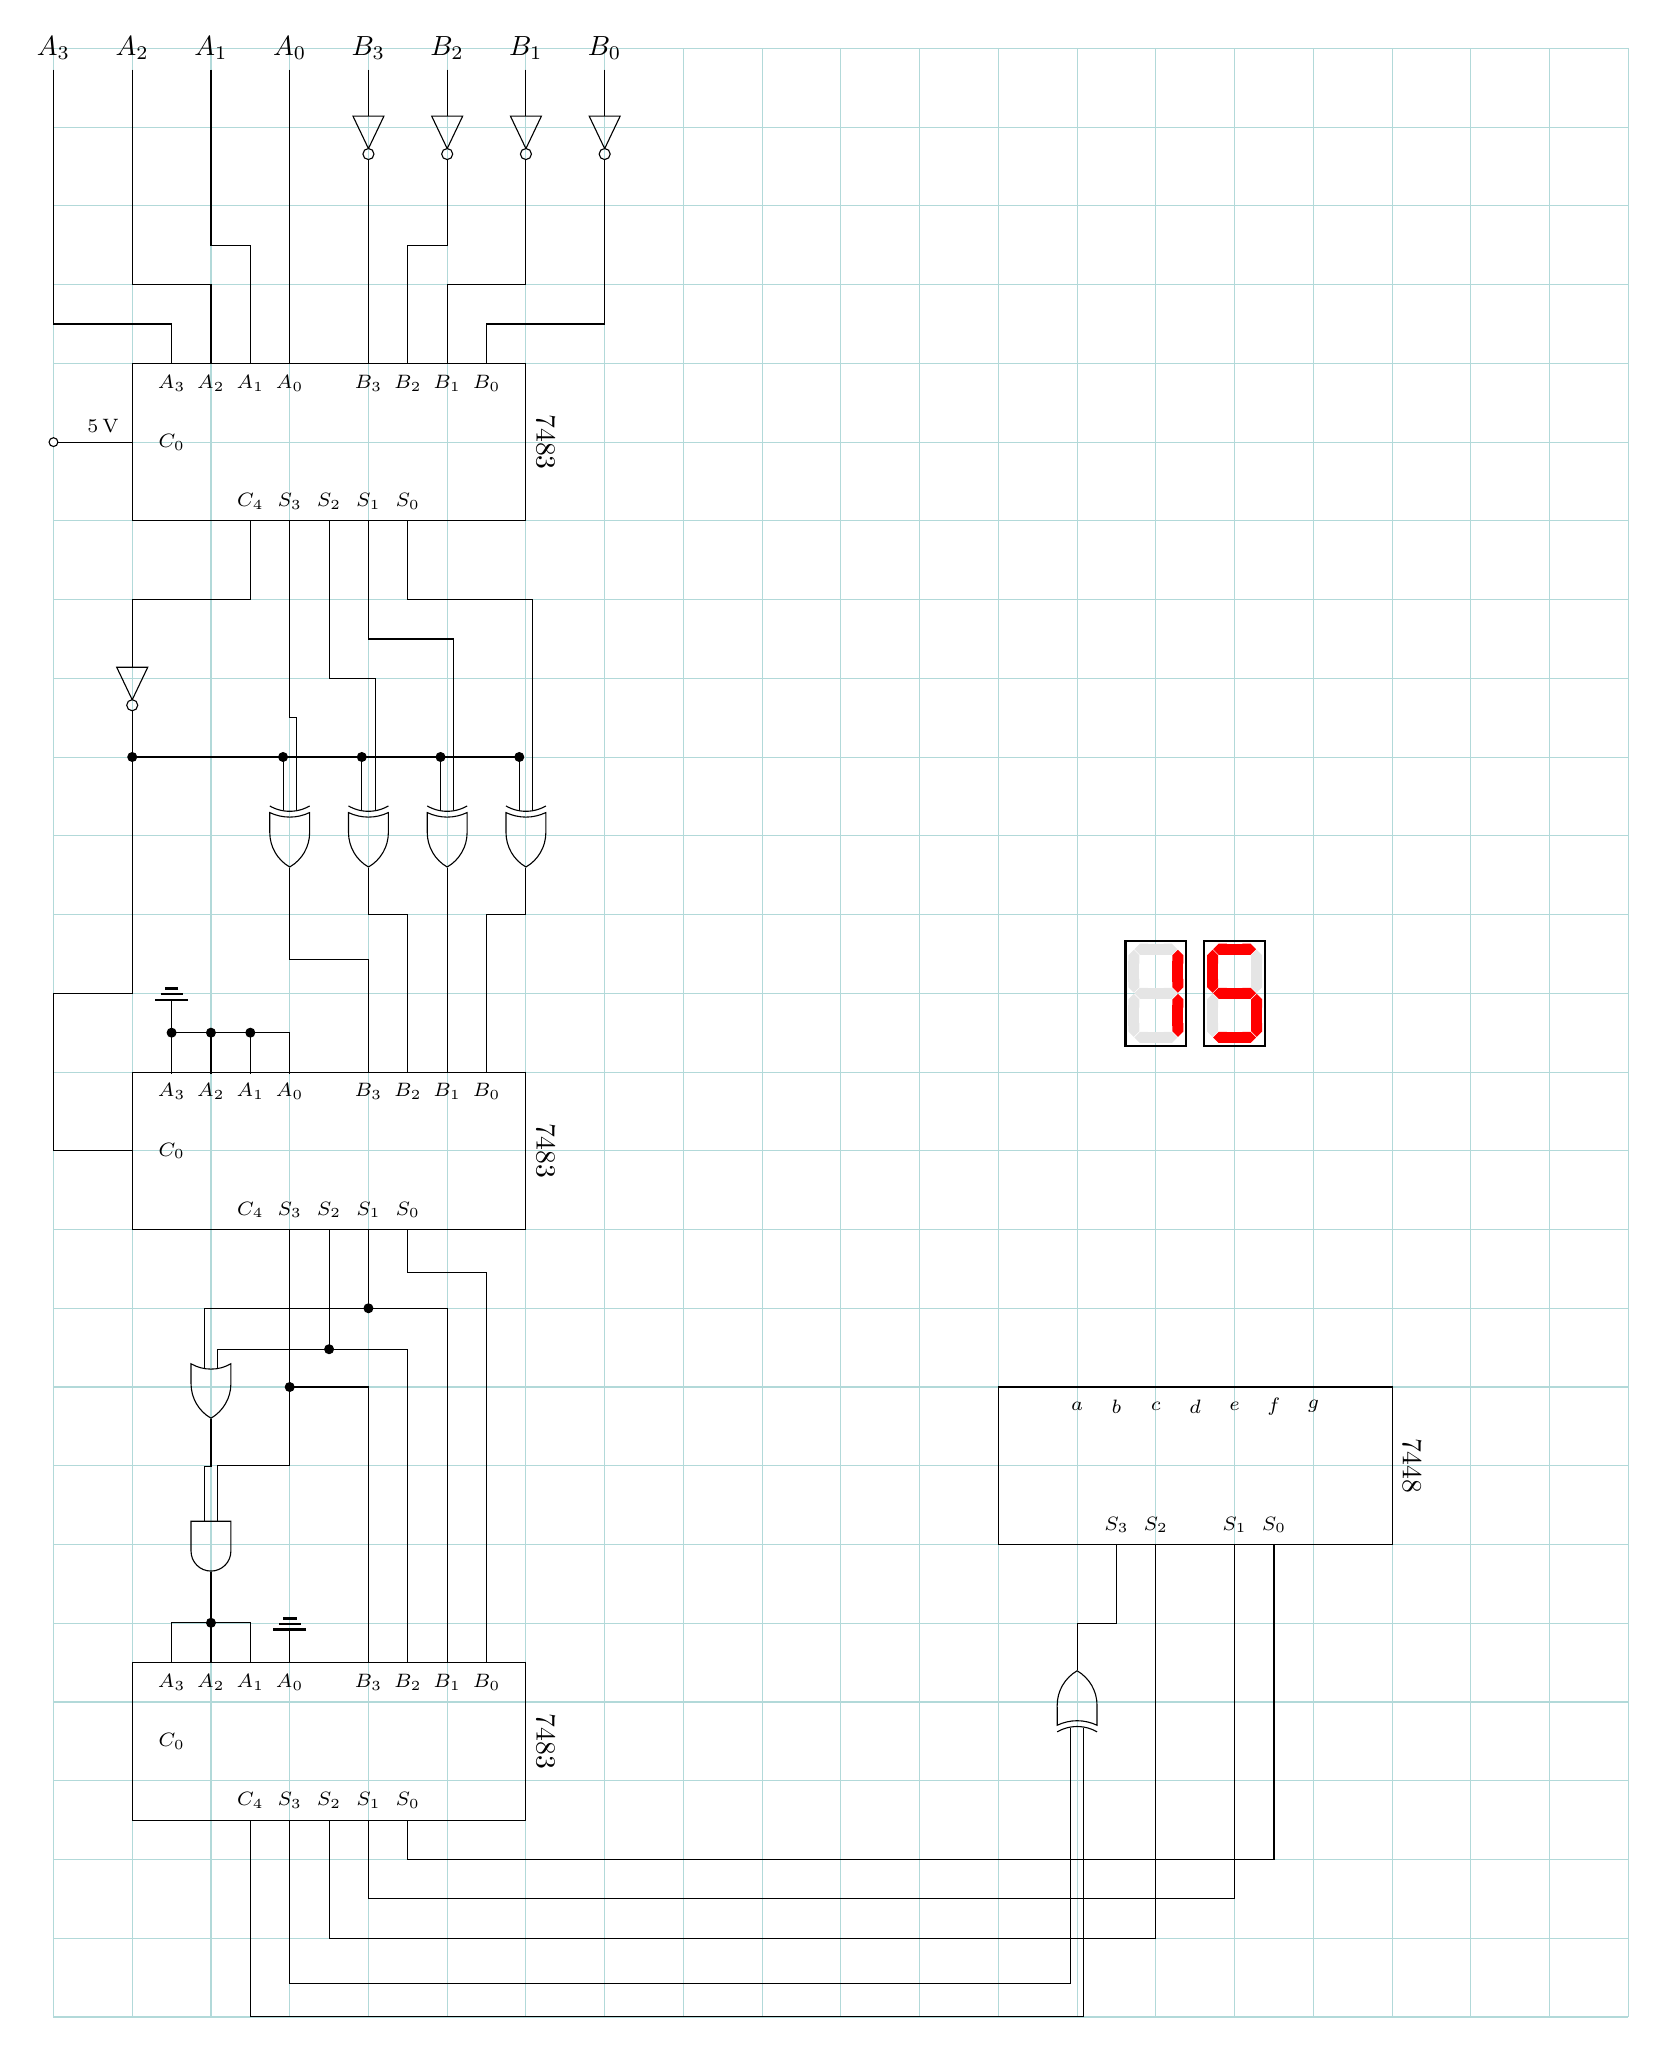
\begin{tikzpicture}
	\draw [help lines] (0,0) grid (20,-25);

	\node (A3) at (0,0)      {$A_3$};
	\node (A2) [right of=A3] {$A_2$};
	\node (A1) [right of=A2] {$A_1$};
	\node (A0) [right of=A1] {$A_0$};

	\node (B3) [right of=A0] {$B_3$};
	\node (B2) [right of=B3] {$B_2$};
	\node (B1) [right of=B2] {$B_1$};
	\node (B0) [right of=B1] {$B_0$};

	\node ('B3) [not gate US, draw, rotate=-90] at (4,-1)     {};
	\node ('B2) [not gate US, draw, rotate=-90, above of='B3] {};
	\node ('B1) [not gate US, draw, rotate=-90, above of='B2] {};
	\node ('B0) [not gate US, draw, rotate=-90, above of='B1] {};

	\draw (B3) -- ('B3.input);
	\draw (B2) -- ('B2.input);
	\draw (B1) -- ('B1.input);
	\draw (B0) -- ('B0.input);

	% Full Adder (1)

	\draw[black,thin] (1,-4) rectangle ++(5,-2);
	\node (AddA3) [font=\scriptsize] at (1.5, -4.25) {$A_3$};
	\node (AddA2) [font=\scriptsize] at (2, -4.25)   {$A_2$};
	\node (AddA1) [font=\scriptsize] at (2.5, -4.25) {$A_1$};
	\node (AddA0) [font=\scriptsize] at (3, -4.25)   {$A_0$};
	\node (AddB3) [font=\scriptsize] at (4, -4.25)   {$B_3$};
	\node (AddB2) [font=\scriptsize] at (4.5, -4.25) {$B_2$};
	\node (AddB1) [font=\scriptsize] at (5, -4.25)   {$B_1$};
	\node (AddB0) [font=\scriptsize] at (5.5, -4.25) {$B_0$};
	\node (AddC0) [font=\scriptsize] at (1.5, -5)    {$C_0$};
	\node (AddC4) [font=\scriptsize] at (2.5, -5.75) {$C_4$};
	\node (AddS3) [font=\scriptsize] at (3, -5.75)   {$S_3$};
	\node (AddS2) [font=\scriptsize] at (3.5, -5.75) {$S_2$};
	\node (AddS1) [font=\scriptsize] at (4, -5.75)   {$S_1$};
	\node (AddS0) [font=\scriptsize] at (4.5, -5.75) {$S_0$};
	\node (17483) [rotate=-90]       at (6.25, -5)   {$7483$};

	\draw [shorten >=0.5] (A3) -- ++(0, -3.5) -| (AddA3);
	\draw [shorten >=0.5] (A2) -- ++(0, -3)   -| (AddA2);
	\draw [shorten >=0.5] (A1) -- ++(0, -2.5) -| (AddA1);
	\draw [shorten >=0.5] (A0) -- (AddA0);

	\draw [shorten >=0.5] ('B3.output) -- (AddB3);
	\draw [shorten >=0.5] ('B2.output) -- (5, -2.5) -| (AddB2);
	\draw [shorten >=0.5] ('B1.output) -- (6, -3)   -| (AddB1);
	\draw [shorten >=0.5] ('B0.output) -- (7, -3.5) -| (AddB0);

	\node [ocirc](C0) at (0,-5) {};
	\draw [shorten >=6] (C0.east) -- (AddC0) node[midway, above, font=\scriptsize] {$\qty{5}{V}$};

	\node ('AddC4) [not gate US, draw, rotate=-90] at (1,-8)                          {};
	\node (Xor3) [xor gate US, draw, rotate=-90, logic gate inputs=nn] at (3, -10)    {};
	\node (Xor2) [xor gate US, draw, rotate=-90, logic gate inputs=nn, above of=Xor3] {};
	\node (Xor1) [xor gate US, draw, rotate=-90, logic gate inputs=nn, above of=Xor2] {};
	\node (Xor0) [xor gate US, draw, rotate=-90, logic gate inputs=nn, above of=Xor1] {};

	\draw [shorten <=0.5] (AddC4) -- ++(0,-1.25) -  | ('AddC4.input) {};
	\draw [shorten <=0.5] (AddS3) -- ++(0, -2.75) - | (Xor3.input 1) {};
	\draw [shorten <=0.5] (AddS2) -- ++(0, -2.25) - | (Xor2.input 1) {};
	\draw [shorten <=0.5] (AddS1) -- ++(0, -1.75) - | (Xor1.input 1) {};
	\draw [shorten <=0.5] (AddS0) -- ++(0, -1.25) - | (Xor0.input 1) {};

	\draw ('AddC4.output) -- ++(0, -0.58) node[circ]    {} -| node[circ] {} (Xor3.input 2) {};
	\draw ('AddC4.output) -- ++(0, -0.58) -| node[circ] {} (Xor2.input 2) {};
	\draw ('AddC4.output) -- ++(0, -0.58) -| node[circ] {} (Xor1.input 2) {};
	\draw ('AddC4.output) -- ++(0, -0.58) -| node[circ] {} (Xor0.input 2) {};

	% Full Adder (2)

	\draw[black,thin] (1,-13) rectangle ++(5,-2);
	\node (Add1A3) [font=\scriptsize] at (1.5, -13.25) {$A_3$};
	\node (Add1A2) [font=\scriptsize] at (2, -13.25)   {$A_2$};
	\node (Add1A1) [font=\scriptsize] at (2.5, -13.25) {$A_1$};
	\node (Add1A0) [font=\scriptsize] at (3, -13.25)   {$A_0$};
	\node (Add1B3) [font=\scriptsize] at (4, -13.25)   {$B_3$};
	\node (Add1B2) [font=\scriptsize] at (4.5, -13.25) {$B_2$};
	\node (Add1B1) [font=\scriptsize] at (5, -13.25)   {$B_1$};
	\node (Add1B0) [font=\scriptsize] at (5.5, -13.25) {$B_0$};
	\node (Add1C0) [font=\scriptsize] at (1.5, -14)    {$C_0$};
	\node (Add1C4) [font=\scriptsize] at (2.5, -14.75) {$C_4$};
	\node (Add1S3) [font=\scriptsize] at (3, -14.75)   {$S_3$};
	\node (Add1S2) [font=\scriptsize] at (3.5, -14.75) {$S_2$};
	\node (Add1S1) [font=\scriptsize] at (4, -14.75)   {$S_1$};
	\node (Add1S0) [font=\scriptsize] at (4.5, -14.75) {$S_0$};
	\node (27483) [rotate=-90]       at (6.25, -14)    {$7483$};

	\draw [shorten >=6] ('AddC4.output) -- ++(0, -3.58) -- ++(-1, 0) |- (Add1C0) {};
	\draw [shorten >=0.5] (Xor3.output) -- ++(0, -1.17) -| (Add1B3)              {};
	\draw [shorten >=0.5] (Xor2.output) -- ++(0, -0.59) -| (Add1B2)              {};
	\draw [shorten >=0.5] (Xor1.output) -- (Add1B1)                              {};
	\draw [shorten >=0.5] (Xor0.output) -- ++(0, -0.59) -| (Add1B0)              {};

	\node[ground, draw, rotate=180] (Add1A) at (1.5, -12.5) {};
	\node[circ] at (Add1A) {};

	\draw (Add1A) -- (Add1A3)   {};
	\draw (Add1A) -| node[circ]{} (Add1A2) {};
	\draw (Add1A) -| node[circ]{} (Add1A1) {};
	\draw (Add1A) -| (Add1A0) {};

	\node (Or1) [or gate US, draw, rotate=-90, logic gate inputs=nn] at (2, -17)   {};
	\node (And1) [and gate US, draw, rotate=-90, logic gate inputs=nn] at (2, -19) {};

	% Full Adder (3)

	\draw [black,thin] (1,-20.5) rectangle ++(5,-2);
	\node (Add2A3) [font=\scriptsize] at (1.5, -20.75) {$A_3$};
	\node (Add2A2) [font=\scriptsize] at (2, -20.75)   {$A_2$};
	\node (Add2A1) [font=\scriptsize] at (2.5, -20.75) {$A_1$};
	\node (Add2A0) [font=\scriptsize] at (3, -20.75)   {$A_0$};
	\node (Add2B3) [font=\scriptsize] at (4, -20.75)   {$B_3$};
	\node (Add2B2) [font=\scriptsize] at (4.5, -20.75) {$B_2$};
	\node (Add2B1) [font=\scriptsize] at (5, -20.75)   {$B_1$};
	\node (Add2B0) [font=\scriptsize] at (5.5, -20.75) {$B_0$};
	\node (Add2C0) [font=\scriptsize] at (1.5, -21.5)    {$C_0$};
	\node (Add2C4) [font=\scriptsize] at (2.5, -22.25) {$C_4$};
	\node (Add2S3) [font=\scriptsize] at (3, -22.25)   {$S_3$};
	\node (Add2S2) [font=\scriptsize] at (3.5, -22.25) {$S_2$};
	\node (Add2S1) [font=\scriptsize] at (4, -22.25)   {$S_1$};
	\node (Add2S0) [font=\scriptsize] at (4.5, -22.25) {$S_0$};
	\node (37483) [rotate=-90]       at (6.25, -21.5)    {$7483$};

	\draw [shorten <=0.6, shorten >=0.6] (Add1S0) -- ++(0, -0.8) -| (Add2B0)  {};
	\draw [shorten <=0.6, shorten >=0.6] (Add1S1) -- ++(0, -1.25) -| (Add2B1) {};
	\draw [shorten <=0.6, shorten >=0.6] (Add1S2) -- ++(0, -1.77) -| (Add2B2) {};
	\draw [shorten <=0.6, shorten >=0.6] (Add1S3) -- ++(0, -2.25) node[circ]  {} -| (Add2B3) {};

	\draw [shorten <=0.6] (Add1S1) -- ++(0, -1.25) node[circ]         {} -| (Or1.input 2) {};
	\draw [shorten <=0.6] (Add1S2) -- ++(0, -1.77) node[circ]         {} -| (Or1.input 1) {};
	\draw (Or1.output) -| ++(0, -0.6) -| (And1.input 2)               {};
	\draw [shorten <=0.6] (Add1S3) -- ++(0, -3.25)  -| (And1.input 1) {};

	\draw [shorten >=0.5] (And1.output) -- ++(0, -0.65) node[circ] {} -| (Add2A3) {};
	\draw [shorten >=0.5] (And1.output) -- ++(0, -0.65) -| (Add2A2) {};
	\draw [shorten >=0.5] (And1.output) -- ++(0, -0.65) -| (Add2A1) {};
	\node [ground, rotate=180] at (3, -20.5) {};

	% Seven segment driver
	
	\draw [black,thin] (12,-17) rectangle ++(5,-2);
	\node (a) [font=\scriptsize] at (13, -17.25)    {$a$};
	\node (b) [font=\scriptsize] at (13.5, -17.25)  {$b$};
	\node (c) [font=\scriptsize] at (14, -17.25)    {$c$};
	\node (d) [font=\scriptsize] at (14.5, -17.25)  {$d$};
	\node (e) [font=\scriptsize] at (15, -17.25)    {$e$};
	\node (f) [font=\scriptsize] at (15.5, -17.25)  {$f$};
	\node (g) [font=\scriptsize] at (16, -17.25)    {$g$};
	\node (S3) [font=\scriptsize] at (13.5, -18.75) {$S_3$};
	\node (S2) [font=\scriptsize] at (14, -18.75)   {$S_2$};
	\node (S1) [font=\scriptsize] at (15, -18.75)   {$S_1$};
	\node (S0) [font=\scriptsize] at (15.5, -18.75) {$S_0$};
	\node (7448) [rotate=-90]       at (17.25, -18) {$7448$};

	\draw [shorten <=0.5, shorten >=0.5] (S0) -- ++(0, -4.25) -| (Add2S0) { };
	\draw [shorten <=0.5, shorten >=0.5] (S1) -- ++(0, -4.75) -| (Add2S1) { };
	\draw [shorten <=0.5, shorten >=0.5] (S2) -- ++(0, -5.25) -| (Add2S2) { };

	\node (Xor5) [xor gate US, draw, rotate=90, logic gate inputs=nn] at (13, -21) { };

	\draw (S3) [shorten <=0.5] -- ++(0, -1.25) -| (Xor5.output) { };
	\draw (Xor5.input 1) [shorten >=0.5] -- ++(0, -3.25) -| (Add2S3) { };
	\draw (Xor5.input 2) [shorten >=0.5] -- ++(0, -3.67) -| (Add2C4) { };

	\node (AnodeDisplay) [seven segment val=1 dot none box on] at (14, -12) { };
	\node (CathodeDisplay) [seven segment val=5 dot none box on] at (15, -12) { };

\end{tikzpicture}
\end{document}
